\section{Experimentación General}

\par{El objetivo de esta sección es comparar las heurísticas implementadas,
tanto en performance como en optimalidad, entre sí y con el algoritmo exacto.
Los archivos $super\_test.cpp$ y $super\_opt.cpp$ en la carpeta $codigo$
implementan esas pruebas respectivamente. Son iguales a los específicos de cada
heurística pero en lugar de evaluar una sola (o variantes de la misma) evalúa
y compara todas juntas. En cada caso, los algoritmos evaluados fueron los
siguientes:}\\

${\color{yellow}\bullet}$ Algoritmo Exacto con poda\\

${\color{red}\bullet}$ Heurística constructiva golosa\\

${\color{green}\bullet}$ Heurística de búsqueda Local con V=2\\

${\color{cyan}\bullet}$ Heurística de búsqueda Local con V=3\\

${\color{blue}\bullet}$ Heurística de búsqueda Tabú con V=1\\

${\color{violet}\bullet}$ Heurística de búsqueda Tabú con V=2\\

\par{Las heurísticas de búsqueda parten de la solución vacía.
No nos pareció pertinente comparar estos algoritmos con la versión sin
poda del algoritmo exacto ya que sólo servía para compararlo con su contraparte
con poda. No era la idea presentarlo como un algoritmo más, sino que se
implementó para ver que efectivamente la poda disminuía los tiempos de
ejecución. Ya que no hubo mejoras considerables con la heurística de búsqueda
tabú con $V$=3 respecto a su variante con $V$=2\footnote{ver sección
\textbf{experimentación} de \textbf{búsqueda tabú}}, se determinó no evaluar
ambas y, ya que los tiempos de ejecución de la variante con $V$=3 fueron muy
superiores a los de la variante con $V$=2, se eligió esta última.
Tampoco se vieron diferencias considerables al variar el tamaño de la lista $T$
de la búsqueda tabú, por lo que se dejó constante en $n$, al igual que la
cantidad máxima de iteraciones $I$.}\\

\par{Después de
algunas pruebas iniciales se determinó que la heurística de búsqueda local con
$V$=1 era idéntica a la heurística golosa. Tiene sentido si pensamos que
ambas parten de la solución vacía. En cada iteración, la heurística golosa
agrega el nodo que más incrementa la frontera, mientras que búsqueda local,
de las soluciones vecinas a la actual (una solución es vecina si se le agrega o
se le saca un nodo) toma la mejor. Como se parte de la solución vacía, las
soluciones vacinas son todas las que tienen exactamente un nodo, es decir las
mismas que se pueden formar después de la primera iteración de la heurística
golosa.}\\

\par{Para evitar que sean tan similares, se intentó que la solución inicial de
búsqueda local sea la solución de la golosa, pero el problema persistió. Al
parecer, la búsqueda local con $V$=1 no pudo mejorar la solución golosa. Es por
esto que la heurística local con $V$=1 tampoco se evalúa. En el siguiente
gráfico (resultante de ejecutar el programa en $golosa$-$local.cpp$) se ve que
la búsqueda local no puede superar a la golosa ya sea que inicie con la solución
vacía, o con la solución devuelta por la heurística golosa.}
\newpage
\begin{center}
\textbf{Gráfico de optimalidad de las heurísticas golosa y de búsqueda\\
local en función de la cantidad de nodos del grafo}
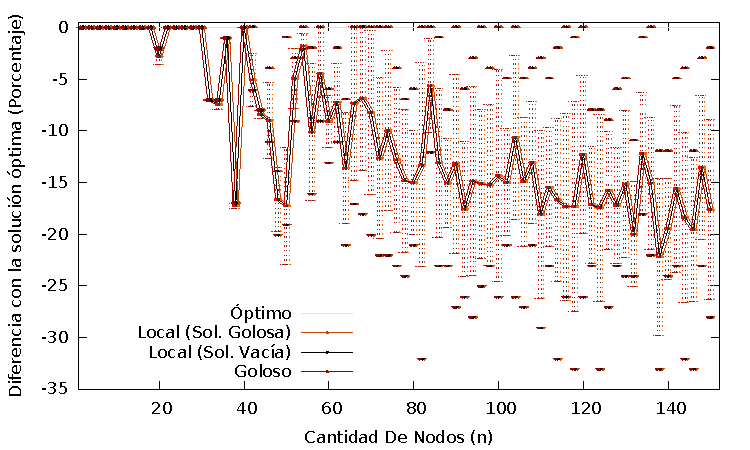
\includegraphics[scale=1.3]{imgs/golosa-local_150_2_10.pdf}
\end{center}

\par{El programa de $golosa-local.cpp$ se corrió con los parámetros $N$ =
150, $s$ = 2 y $k$ = 10. Es decir, para cada $n$ entero par entre 2 y 150, se
generaron 10 grafos aleatorios. Para cada instancia generada se corrieron la
heurística golosa y dos variantes de la búsqueda local con $V$=1. Una a partir
de la solución vacía y otra a partir de la solución obtenida con la heurística
golosa. Como se puede ver, El índice de optimalidad es el mismo para las tres
heurísticas en todos los casos. Incluso coinciden en la varianza, los máximos
y los mínimos.}

\subsection{Performance}

\par{El archivo $super\_test.cpp$ en la carpeta $codigo$ contiene la
implementación del código que mide los tiempos de ejecución de las cinco
heuristicas y del algoritmo exacto. Se ejecutó este programa con $N$ =
150, $s$ = 2 y $k$ = 10. Es decir, para cada $n$ entero par entre 2 y 150, se
generaron 10 grafos aleatorios (con la función $generar\_aristas\_aleatorias$).
Para cada instancia generada se corrieron los seis algoritmos mencionados al
principio de la sección.
En el siguiente gráfico se muestran los resultados obtenidos.}
\newpage
\begin{center}
\textbf{Gráfico de performance general en\\función de la cantidad
de nodos del grafo}
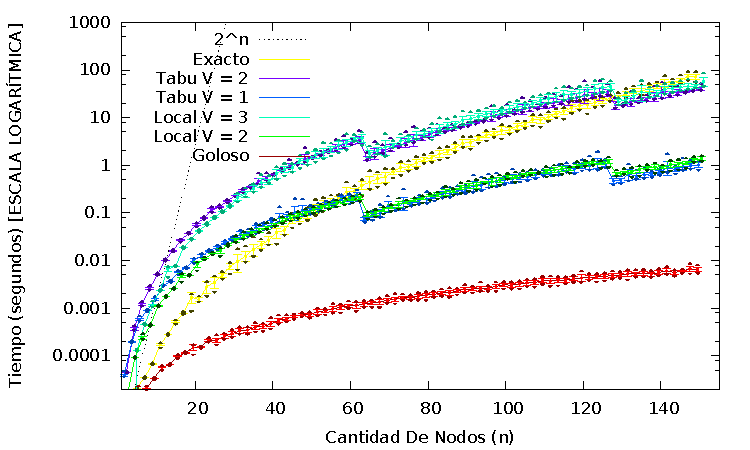
\includegraphics[scale=1.3]{imgs/super_test_150_2_10.pdf}
\end{center}

\par{La curva punteada negra con la etiqueta $2^n$ es la misma que la
graficada en el gráfico de performance del algoritmo exacto, por lo que
debería coincidir más o menos con los tiempos de ejecución de dicho
algoritmo sin poda. Es claro que todas las heurísticas están lejos de alcanzar
tal complejidad.}\\

\par{Debido a los altos tiempos de ejecución del algoritmo exacto (y de las
heurísticas también) nos vimos limitados a testear hasta 150 nodos. A pesar que,
hasta $n$=120 las heurísticas tabú con $V$=2 y local con $V$=3 tienen tiempos de
ejecución superiores al algoritmo exacto, es claro que al incrementar la
cantidad de nodos mucho más, terminará habiendo una mejora considerable (en
cuanto a tiempos de ejecución) de estas heurísticas con respecto al algoritmo
exacto. En este punto ya podemos concluír que para grafos con cantidad de nodos
menor a 120 es preferible usar el algoritmo exacto antes que las heurísticas
tabú con $V$=2 o local con $V$=3, ya que el primero retorna una solución óptima
y tiene menores tiempos de ejecución.}\\

\par{Es notable lo similares que son las curvas definidas por las heurísticas
tabú con $V$=2 y local con $V$=3. En un principio tabú parece ser ligeramente
superior pero a partir de $n$=60, esta pequeña diferencia se invierte. Algo
similar sucede entre las curvas definidas por las heurísticas tabú con $V$=1
y local con $V$=2, donde también la tabú empieza siendo superior, pero luego
pasa a ser inferior a la local.}\\

\par{Otra cosa que llama la atención es la abrupta caída que tienen las cuatro
heurísticas de búsqueda en los grafos con 64 y 128 nodos. Si bien la escala
logarítmica no lo permite ver, esta recaída en los tiempos de ejecución es
de al rededor de la mitad.}

\subsection{Optimalidad}

\par{El archivo $super\_opt.cpp$ en la carpeta $codigo$ contiene la
implementación del código que mide el índice de optimalidad de las cinco
heuristicas. Se ejecutó este programa con $N$ = 150, $s$ = 2 y $k$ = 10. Es
decir, para cada $n$ entero par entre 2 y 150, se generaron 10 grafos
aleatorios (con la función $generar\_aristas\_aleatorias$).
Para cada instancia generada se corrieron los seis algoritmos mencionados al
principio de la sección (Los resultados del algoritmo exacto son siempre
cero. El algoritmo se corre para obtener la máxima frontera de cada instancia
generada y poder calcular el índice de optimalidad de las heurísticas).
En el siguiente gráfico se muestran los resultados obtenidos.}

\begin{center}
\textbf{Gráfico de optimalidad general en\\función de la cantidad
de nodos del grafo}
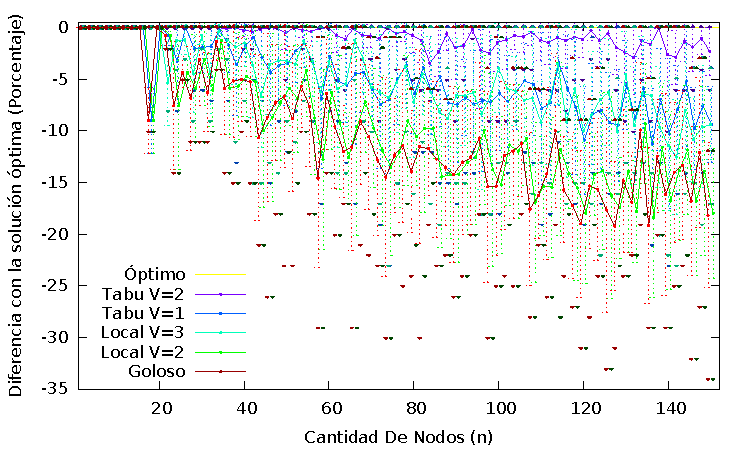
\includegraphics[scale=1.3]{imgs/super_opt_150_2_10.pdf}
\end{center}

\par{Como era de esperarse, la heurística tabú con $V$=2 resultó
ser la más cercana a la recta $y=0$, con un promedio de índice de
optimalidad menor al 5\% y mínimos al rededor del 10\%. Luego le
siguen las heurísticas tabú con $V$=1 y local con $V$=3, con un
promedio de al rededor del 10\% y mínimos entre el 15\% y el 20\%.
Estas dos resultaron ser muy similares en cuanto a optimalidad y
no está del todo claro si alguna es superior a la otra, ya que en
varios puntos se entrelazan. Finalmente, también muy similares entre
sí, las heurísticas golosa y local con $V$=2, con promedios al
rededor del 15\% y mínimos de más del 30\%. El siguiente gráfico
se realizó con los mismos datos pero sin la varianza, además de
reducir el rango vertical para tener una visión más detallada de
las curvas promedio.}
\newpage
\begin{center}
\textbf{Gráfico de optimalidad general en función de\\la cantidad
de nodos del grafo (sin varianza y ampliado)}
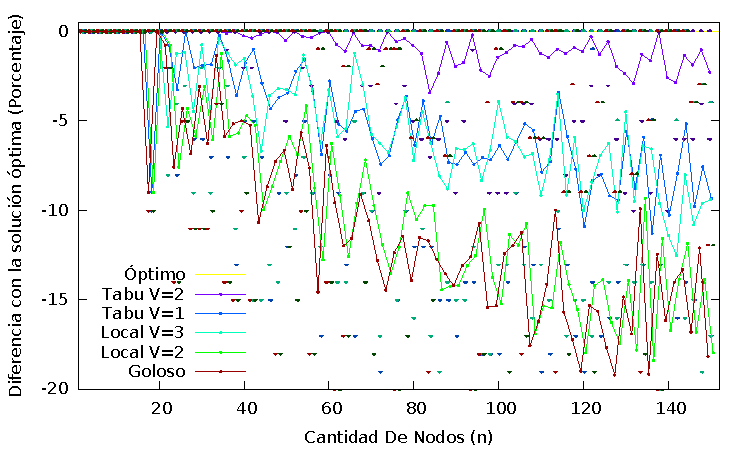
\includegraphics[scale=1.3]{imgs/super_opt_150_2_10_p.pdf}
\end{center}

\par{En este segundo gráfico se pueden observar mejor las relaciones entre las
heurísticas; los segmentos de las varianzas entorpecían mucho la vista y por eso
se decidió quitarlas. A partir de este gráfico y del de performance, podemos
concuír que simepre es mejor utilizar la heurística tabú con $V$=2 antes que la
local con $V$=2, ya que los tiempos de ejecución eran muy similares (de hecho,
la tabú era ligeramente superior a partir de $n$=60) pero la primera obtiene
resultados mucho mejores. Si las opciones son tabú con $V$=1 y local con $V$=3,
también es preferible la opción tabú, ya que ambas tienen resultados similares
pero los tiempos de ejecución de la versión tabú son al menos 10 veces menores
(recordar que el gráfico de performance está en escala logarítmica). Tampoco
es recomendable utilizar la local con $V$=2 frente a la golosa, una vez más
estas dos heurísticas obtienen resultados similares, pero los tiempos de
ejecución de la heurística golosa son muchísimo menores.}\\

\par{Antes de comenzar los tests, se quitó la heurística de búsqueda local con
$V$=1 por ser exactamente igual a la heurística golosa en cuanto a optimalidad.
Sin embargo se ve que su variante con $V$=2 no difiere mucho de la golosa, por
lo tanto tampoco debería diferir mucho de la variante con $V$=1. Si recordamos
el gráfico de optimalidad de búsqueda local\footnote{ver sección
\textbf{experimentación} de \textbf{búsqueda local}} eso es exactamente lo que
sucede.}
